%\documentclass[english,twoside]{article}
\documentclass[english,twoside]{labmanual} 
%labmanual.cls is a modified version of article.cls, tweaked to handle \part{} differently

%% LyX 1.1 created some parts of this file.  For more info, see http://www.lyx.org/.
%% Do not edit unless you really know what you are doing.

\usepackage[T1]{fontenc}
\usepackage[nomarginpar]{geometry}
\usepackage{tocloft} %Allow us to leave page numbers for Parts out of table of contents
\cftpagenumbersoff{part} %No page numbers for Parts out of table of contents
\renewcommand{\cftsecdotsep}{\cftsubsecdotsep}
%\usepackage{newclude} %Allows use of /include*{}
%DANGER DANGER: newclude is NOT compatible with package xr, used for external references.
\geometry{verbose,letterpaper}
\usepackage{fancyhdr}
\usepackage{babel}
\setlength\parskip{\medskipamount}
\setlength\parindent{0pt}
\usepackage{graphicx}
\usepackage{wrapfig}
%\usepackage{epstopdf} %this package apparently allows pdflatex to work on this document, since all we use are eps figures.
\usepackage{comment}
\usepackage{esvect}
\usepackage{amsmath} %uncommented by MT 5/2015, used in "E near charged rod"
\usepackage{mathtools} %added by MT 6/2015, for access to dcases environment in finding_v_from_e
\usepackage{tabularx} %added by MT 6/2015, for fixed width columns, used in rc_circuits
\usepackage{microtype}
\usepackage{titlesec}
\usepackage{xr}

%For fixed width columns:
\newcolumntype{L}[1]{>{\raggedright\arraybackslash}p{#1}}
\newcolumntype{C}[1]{>{\centering\arraybackslash}p{#1}}
\newcolumntype{R}[1]{>{\raggedleft\arraybackslash}p{#1}}


\addtolength{\oddsidemargin}{1.0cm} %without these two lines, larger margin is on the OUTSIDE.  We want the larger edge on the INSIDE, to allow room for the three hole punches
\addtolength{\evensidemargin}{-1.0cm}

\setlength\topmargin{0.2in}
\addtolength{\hoffset}{-1.0cm}
\addtolength{\textwidth}{2.0cm}
\addtolength{\voffset}{-1.5cm} %This line is apparently needed on some versions of MikTex XeLatex.  Comment out if your pages appear shifted too high.
\addtolength{\textheight}{3.5cm}
% define a strut for extra vertical space in tables.
\newcommand{\hi}{\rule[-2mm]{0mm}{6mm}}

\pagestyle{fancy}
%\fancyhead[LE,RO]{\slshape \rightmark} %This is the default for fancy page style
%\fancyhead[LO,RE]{\slshape \leftmark}
\fancyhead[LO,RE]{\slshape \rightmark} 
\fancyhead[LE,RO]{\slshape \leftmark} % Reversed LE, RO to  LO,RE to make headers come out correctly on even/odd pages



%%%%%%%%%%%%%%%%%%%%%%%%%%%%%% LyX specific LaTeX commands.
\providecommand{\LyX}{L\kern-.1667em\lower.25em\hbox{Y}\kern-.125emX\@}
\newenvironment{LyXParagraphIndent}[1]%
{
  \begin{list}{}{%
    \setlength\topsep{0pt}%
    \addtolength{\leftmargin}{#1}
    \setlength\parsep{0pt plus 1pt}%
  }
  \item[]
}
{\end{list}}
%% Special footnote code from the package 'stblftnt.sty'
%% Author: Robin Fairbairns -- Last revised Dec 13 1996
\makeatletter
\let\SF@@footnote\footnote
\def\footnote{\ifx\protect\@typeset@protect
    \expandafter\SF@@footnote
  \else
    \expandafter\SF@gobble@opt
  \fi
}
\expandafter\def\csname SF@gobble@opt \endcsname{\@ifnextchar[%]
  \SF@gobble@twobracket
  \@gobble
}
\edef\SF@gobble@opt{\noexpand\protect
  \expandafter\noexpand\csname SF@gobble@opt \endcsname}
\def\SF@gobble@twobracket[#1]#2{}
\makeatother


%I make use of some latex features to manage the section numbers. To use those you have to insert the following lines into the latex preamble (before the %"\begin{document}" command).

% two new commands to do labelling. - gpg 12/4/13
\newcommand{\customlabel}[2]{%
\protected@write \@auxout {}{\string \newlabel {#1}{{#2}{}}}}

\newcommand{\actlabel}[1]{%
\protected@write \@auxout {}{\string \newlabel {#1}{{\arabic{activity}}{}}}}

\newcommand{\makelabheader}
%{Name: \rule{2.0in}{0.1pt}\hfill{}Section: \rule{1.0in}{0.1pt}\hfill{}Date: \rule{1.0in}{0.1pt}}
{Name: \rule{2.0in}{0.1pt}\hfill{}Lab Partner(s): \rule{3.0in}{0.1pt}}

%\newcommand{\dir131}{../../131/StudentGuideModule1} %This does not work, because commands can only be made of numeric characters, not numbers.

%A new command for putting a box around a paragraph:
\newenvironment{newboxed} %maybe there's a better way to do this.  I just cribbed from the web. --MT
    {\begin{center}
    \begin{tabular}{|p{0.9\textwidth}|}
    \hline\\
    }
    { 
    \\\\\hline
    \end{tabular} 
    \end{center}
    }

\newcounter{activity}

%  The following command, \answerspace, should be used to replace \vspace.
%  \vspace{} is not ideal for an answer space for students, for two reasons:
%  1. It can be ignored if it comes at the end of a page, and
%  2. The spacing is exact, and Latex will not stretch or compress it at all to make things fit on a page, which means
%  that other things WILL get stretched or compressed to make things fit, which means those other things will 
%  end up looking bad, and leading to a lot of underfull \vbox warnings.
%  \answerspace fixes both of those problems, specifically allowing the space to grow to up to twice the stated size.
\newcommand{\answerspace}[1]{\vspace*{#1 plus #1}}

%  The next several lines implement \includelab, which replaces \include.
%  Usage is \includelab{1}{file} to include it, or \includelab{0}{file} to NOT include it.  
%  But all 0's can be overridden by writing \includealllabstrue in the master.tex file, which is easier than deleting 
%  fifty individual `%' signs and then remembering to put them all back, which is what you had to do before.
%  \includeonly still works as you expect it to.
\newif\ifincludealllabs
\newcommand{\includelab}[2]{
	\ifnum#1=1
		\include{#2}
	\else {
		\ifincludealllabs
		 	\include{#2}
		\fi}
	\fi
}
 %all general latex packages, commands, and definitions now here.
\externaldocument{master}

%syntax: \includeonly{lab1,lab2,lab3} with no spaces after the commas.
%\includeonly{biot_savart_law/biot_savart_law, charge_density/charge_density,eoverm/eoverm }
%DANGER: The includeonly statement will make a document that does NOT have sequential page numbers.

\newcommand{\supplementmark}{MT}

\titleformat{\section}{\normalfont\Large\bfseries}{\supplementmark \thesection}{1em}{}
\fancyhead[LO,RE]{\slshape \rightmark} 
\fancyhead[LE,RO]{\slshape \supplementmark \leftmark} % Reversed LE, RO to  LO,RE to make headers come out correctly on even/odd 

\begin{document}

\setcounter{page}{157}  %Set this to desired first page
\setcounter{section}{37} %set this to desired first section number MINUS ONE

%--------------------------------------------
%Put include statements for labs below here.
\section{Music to Our Ears: Standing Waves on Strings}

\makelabheader %(Space for student name, etc., defined in master.tex)

\begin{comment}
This lab was changed A LOT by Matt Trawick, 1/23/2016. Old version is saved as standing_waves_on_strings_old2015.tex.

1. Reduced the length of the background material.  Tightened up some of the exposition.  Also removed the parts that gave students the equation \lambda = 2L/n (twice!), on the grounds that students can figure it out themselves.  IMHO, the entire ``introduction'' part could still be removed and I wouldn't miss it.

2. Format changed to match the usual ``Activity 1'' etc.

3. Uncertainty is now done more consistently; students calculate uncertainty for v_A and v_B, not just v_A.

4. I removed the previous second section (`Part B') which had students change the masses to get different modes.  It's much more natural to change the frequency, and we have the equipment to do it easily.  Also, plotting T vs 1/n^2 seemed really old-timey.  And all for.... calculating the mass density, which you already knew from the scale anyway.

5.  The new section I put in instead (Activity 2) has students get different modes by changing frequency.  (This prepares them better for doing the same thing for the resonance tubes lab.)  I also have them derive, from pictures, the relationship 
f = (v/2L)n, which students always want to just memorize without thinking about it.
\end{comment}

\bigskip

\textbf{Apparatus}
\begin{itemize} [nosep] 
\item  String vibrator 
\item  Sine wave generator
\item  Inelastic braided string
\item  2 clamps
\item  Superpulley
\item  Mounting rod for the superpulley
\item  Mass and hanger set
\item  Precision balance
\item  Tape measure or meter stick
\end{itemize}

\bigskip
\textbf{Introduction}

How do we make musical sounds? To make a sound, we need something that vibrates. If we want to make musical notes you usually need the vibration to
have an almost constant frequency: that means stable pitch. We also want a frequency that can be easily controlled by the player. In electronic
instruments this is done with electric circuits or with clocks and memories. In non-electronic instruments, the stable, controlled vibration is
produced by a standing wave. Here we discuss the way strings work. This is also a good introduction for studying wind instruments, because vibrating
strings are easier to visualise than the vibration of the air in wind instruments, though the math is very similar.

Waves are oscillations in an elastic medium:
\begin{itemize}
\item  your own vocal cords (the medium) vibrating as air is forced over them by your lungs; 
\item  a stretched string (the medium) on a musical instrument vibrating as it is bowed, hammered or plucked; 
\item  pressure oscillations in a column of air (the medium) in a wind instrument, organ pipe or your own oral and nasal cavities.
\end{itemize}

In each case the medium has an equilibrium state, and when displaced or otherwise perturbed from that state, experiences a force which tends to
restore it to equilibrium. For small perturbations, the restoring force is proportional to the displacement and the medium becomes a simple harmonic
oscillator.


\textbf{Background}

\textbf{Standing waves} are produced by the interference of two traveling waves, both of which have the
same wavelength $\lambda$, speed $v$, and amplitude, but travel in opposite directions through the same medium. 
One way to get standing waves is with reflections, such as when a wave traveling along a stretched string reflects off the end.  The reflected wave travels backwards, interfering with the wave traveling forwards to produce a standing wave pattern on the string.  

One characteristic of every standing wave pattern is that there are points along the medium which appear to be standing still. These points,
sometimes described as points of no displacement, are referred to as \textbf{nodes}. Points in between the nodes that undergo the \textit{maximum} displacement between
large positive and large negative values are called \textbf{antinodes}. When a standing wave pattern is established in a medium, the locations of nodes and antinodes remain fixed and don't move; hence the name ``standing'' waves.  A particular arrangement of nodes and antinodes is called a \textbf{mode} of vibration.

The number of nodes and antinodes in a standing wave depends on the frequency of the wave as well as properties of the medium.  
If you drive a stretched string at an arbitrary frequency, you will probably not see any particular mode; many modes will be mixed together, and the overall amplitude will be small.
But, if the tension and the string's length are correctly adjusted to the frequency of the driving vibrator, one vibrational mode will occur at a much
greater amplitude than the other modes.

\begin{wrapfigure}[9]{r}{0.5\textwidth}
\vspace{-0.15in}
    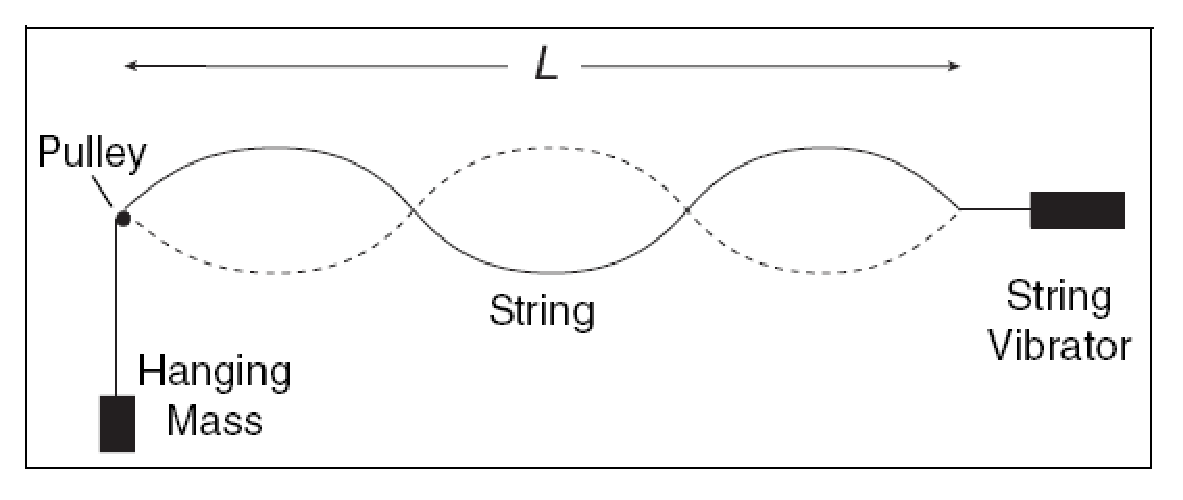
\includegraphics[width=0.5\textwidth]{standing_waves_strings/standing_waves_strings_fig2_tb.eps}
\end{wrapfigure}

\vspace{0.1in}
In this experiment, standing waves are set up in a stretched string by the vibrations of an electrically-driven string vibrator. The tension in the
string equals the weight of the masses suspended over the pulley. You can alter the tension by
changing the masses. 

%\vspace{0.3cm}
%\begin{center}
%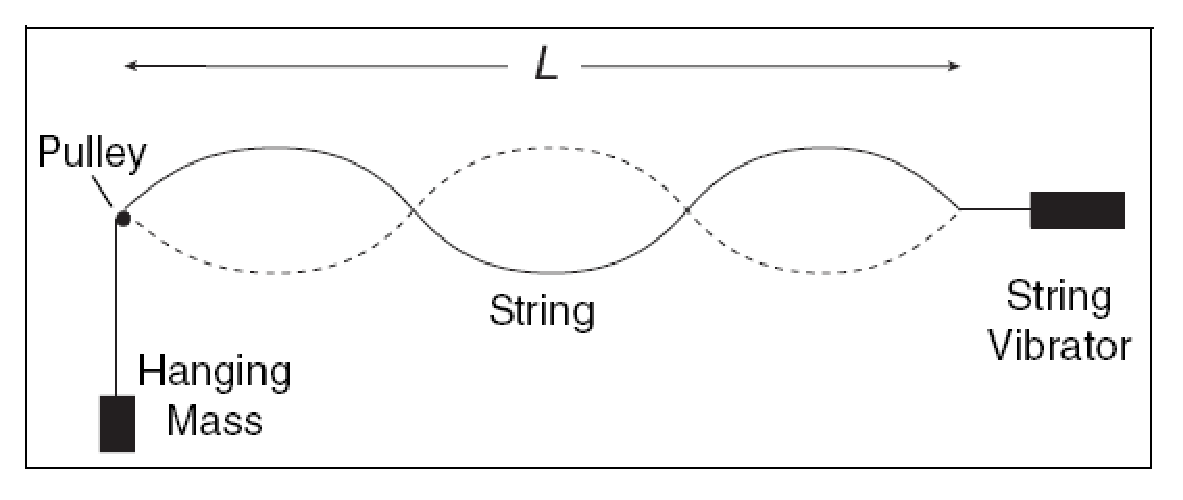
\includegraphics[width=250pt]{standing_waves_strings/standing_waves_strings_fig2_tb.eps}
%%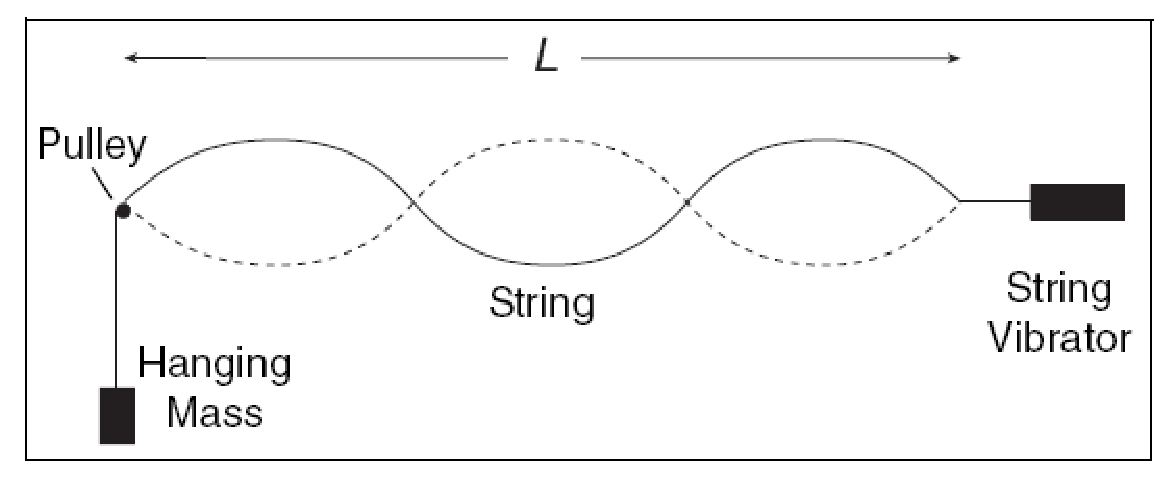
\includegraphics[width=3in]{standing_waves_strings/standing_waves_strings_figure2.eps}
%\end{center}
%\vspace{0.3cm}

The speed of a wave on the string is given by:
\begin{equation*}
v=\sqrt{\frac {T}{\mu }}
\end{equation*}
where $T$ is the tension in the string and $\mu $ is the linear density (mass/length) of the string.  The speed of any wave is also related to its wavelength and frequency by
\begin{equation*}
v=\lambda f.
\end{equation*}


\textbf{Activity 1: Varying the tension and calculating the wave speed}

(a) Clamp the string vibrator and pulley about a meter apart. Attach the string to the vibrating blade, run it over the pulley, and hang about 200 g of mass from it. Cut off the excess string. Measure the distance $L$ from the knot where the string attaches to the string vibrator to the top of the pulley.
%This length $L$ is NOT the total length of the string that you measured in part (a). 

Record the value here, along with the uncertainty: $L$ =

\vspace{0.5cm}
\begin{center}
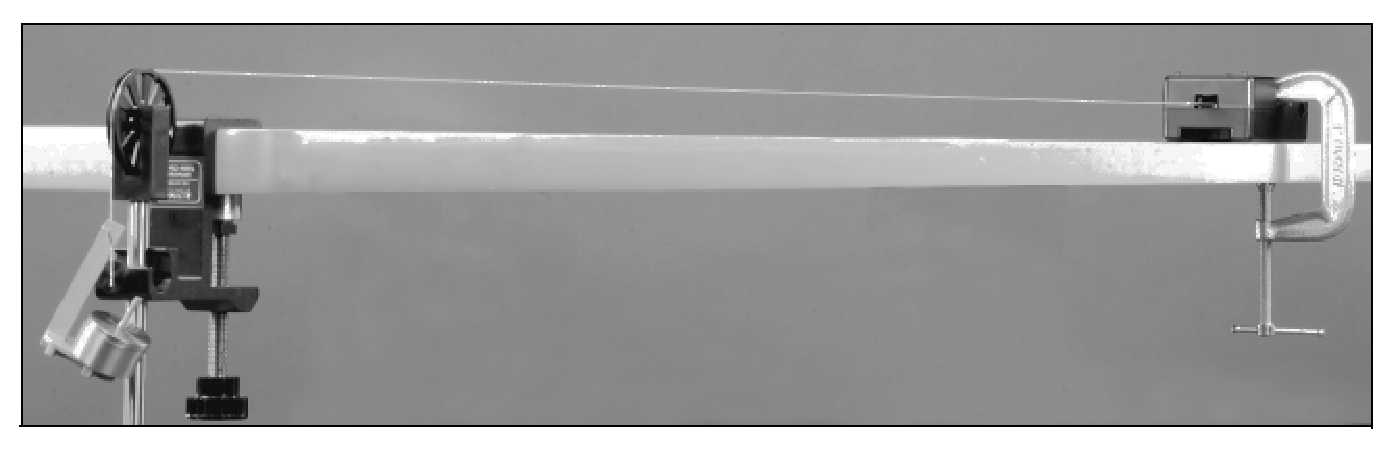
\includegraphics[width=320pt]{standing_waves_strings/standing_waves_strings_fig3_tb.eps}
\end{center}
%\vspace{0.1cm}

Connect the sine wave generator to the string vibrator. (There's a tiny switch in the back of the generator to turn it on.)  Adjust the frequency to 60.0 Hz, and adjust the amplitude to a moderately high value.

Change the tension by adding to or subtracting from the hanging mass so that the string vibrates in 2 segments. Adjust the tension to achieve a ``clean'' node at the center. Also check the end of the vibrating blade; the point where the string attaches should be a node. It is more important to have a good node at the blade than it is to have the largest amplitude possible. However, it is desirable to have the largest amplitude possible while keeping a good node.

(b) Record the best value of the hanging mass, $m$. How much uncertainty is there in that best value? (That is, by how much can you change the hanging mass before you see an effect?) Record the uncertainty too.
\answerspace{2cm}

\pagebreak[2]

(c) Use your mass to calculate the tension $T$ (including the uncertainty) in the string.
\answerspace{2cm}

(d) Measure the exact length of another piece of string several meters long (not the one connected to the string vibrator). Measure the mass of the
string and calculate the linear density $\mu$ (mass/length).  
%(If your balance is not precise enough to measure that length of string, use a longer piece of string.)  
Be sure to estimate the uncertainties in both the mass and the length, bearing in mind that the string can stretch. What is the resulting uncertainty in $\mu$?  (For help with uncertainties, refer to Appendix \ref{uncertainty}.)
\answerspace{4.5cm}

\pagebreak[3]

(e) Calculate the speed $v_A$ of the wave from your observed values of tension
$T$ and linear density $\mu$. Record your calculated value with the uncertainty and the correct number of significant
figures.
\answerspace{4cm}

(f) Calculate the speed $v_B$ from the wavelength ($\lambda $) and frequency ($f$).  What are your uncertainties in $\lambda$ and $f$?  What is your uncertainty in $v_B?$
\answerspace{4cm}

(g) Compare the two values of speed, $v_A$ and $v_B$.  Are the two consistent, to within the uncertainties you calculated?  That is, do their ranges overlap?  (If not, you have some explaining to do....) 
\answerspace{3cm}

\pagebreak[2]
\textbf{Activity 2: Vibrational modes at different frequencies}

\textit{For this part, keep the same string length as in Activity 1, and keep about 200 grams on the end of the string.}

(a) In Activity 1, the standing wave on the string had one node in the middle, dividing the string into $n=2$ vibrating segments.  This means that the standing wave had $n=2$ antinodes.  Change the frequency to find both higher and lower values of $f$ that produce standing waves with different numbers of antinodes.  Record your results in the table below.
\begin{center} 
{\renewcommand{\arraystretch}{1.5}
\begin{tabular}{|c|C{0.8in}|} 
\hline \boldmath$n$ & \boldmath$f$ \textbf{(Hz)} \\ 
\hline 1 &  \\ 
\hline 2 &  \\ 
\hline 3 &  \\ 
\hline 4 &  \\ 
\hline 5 &  \\ 
\hline 6 &  \\ 
\hline 7 &  \\ 
\hline 
\end{tabular} 
}
\end{center}

(\textit{You may need to adjust the amplitude knob to keep the standing wave a reasonable size.  Also, don't worry if the last few modes are too hard to see.  Finally, there's a weird resonance within the string vibrator itself that makes it wonky around 150 Hz; just ignore that and skip past it if necessary.})

\pagebreak[3]

(b) On the lines below, draw pictures of the first three standing wave modes you found.  For each drawing, write the relationship between the half wavelength $\frac{1}{2}\lambda$ and the string length $L$.

\begin{center}
$n=1$: 
\raisebox{-0.15in}{\rule{3pt}{0.4in}}\raisebox{.05in}{\rule{2.5in}{0.1pt}}\raisebox{-0.15in}{\rule{3pt}{0.4in}}
\hspace{0.3in}$\frac{1}{2}\lambda=$

$n=2$:
\raisebox{-0.15in}{\rule{3pt}{0.4in}}\raisebox{.05in}{\rule{2.5in}{0.1pt}}\raisebox{-0.15in}{\rule{3pt}{0.4in}}
\hspace{0.3in}$\frac{1}{2}\lambda=$

$n=3$:
\raisebox{-0.15in}{\rule{3pt}{0.4in}}\raisebox{.05in}{\rule{2.5in}{0.1pt}}\raisebox{-0.15in}{\rule{3pt}{0.4in}}
\hspace{0.3in}$\frac{1}{2}\lambda=$
\end{center}
%axes

(c) From your three pictures above, write a general equation relating $\lambda$ and $L$ for each possible value of $n$.
\answerspace{2cm}

(d) Using the relationship between $\lambda$, $f$, and $v$, rewrite your equation in (c) to express the frequency $f$ for each value of $n$, in terms of $n$, $v$, and $L$.
\answerspace{2cm}

(e) If you were to make a graph of $f$ \textit{vs.} $n$, what would be the slope of that graph, in terms of $v$ and $L$?
\answerspace{2cm}

\pagebreak[3]
(f) Plot a graph of your data for $f$ \textit{vs.} $n$ from part (a) using Excel.\footnote{In general, ``plot $A$ \textit{vs.} $B$'' means ``plot $A$ as a function of $B$,'' which implies that thing $B$ should go on the horizontal axis.} Use the LINEST function to determine the slope of the graph and its uncertainty. (See Appendix \ref{excel} for help using Excel's LINEST function.)  Do you want LINEST to estimate the $y$-intercept, or force it to zero?  Record the slope and its uncertainty here.
\answerspace{3cm}



(g) Does the uncertainty in the slope given by LINEST capture \textit{all} sources of uncertainty in your measurement?
\answerspace{2cm}

(h) Using your values from (f), calculate the velocity of the wave and its uncertainty. 
\answerspace{4cm}

(i) Is the velocity you just calculated consistent with the values $v_A$ and $v_B$ you calculated in Activity 1?  
\answerspace{3cm}


%\textbf{Further Investigation}
%
%If a strobe is available, observe the standing wave on a string with the 
%strobe light. Draw a diagram explaining the motion of the string.





\section{Entropy: Is It Possible?}

\begin{comment}
This lab is more of a worksheet than it is a lab.  But I've used versions of if in my 132 classes for a while, so I thought it was time to include it here in the lab manual for others as well.  --Matt Trawick, 1/2016

\end{comment}

\makelabheader %(Space for student name, etc., defined in master.tex)

\vspace{0.2in}
\textbf{Introduction} 

We are all familiar with the idea that a closed system tends to evolve from an ordered state to a disordered state.  For example, when you put cream into a mug of coffee, the cream tends to disperse: the mug evolves from an ``ordered'' state, with seperate regions of pure cream and black coffee, to a ``disordered'' state with the two mixed together.  The reverse process, spontaneous separation back into pure cream and black coffee, will never happen.

We also know intuitively that heat will always flow from a hot object to a cold object: when you put a hot brick in contact with a cold brick, you end up with two luke-warm bricks.  The reverse process, two luke-warm bricks spontaneously evolving to one hot brick and one cold brick, won't happen.  

In both of the examples above, the ``disorder'' (or ``dispersal'') of the system increases.  We quantify that disorder using entropy, $S$, and for any real process, $\Delta S \geq 0$.  In the context of heat transfer, the change in entropy $\Delta S$ of an object is given by 
\begin{displaymath}
\Delta S = \frac{\Delta Q}{T},
\end{displaymath}
where $\Delta Q$ is the heat energy into the object.  

\vspace{0.3 in}
\textbf{Activity 1: Just Heat Transfer}

Consider the previous example of the hot and cold bricks, illustrated below.

\begin{center}
\vspace{-0.2 in}
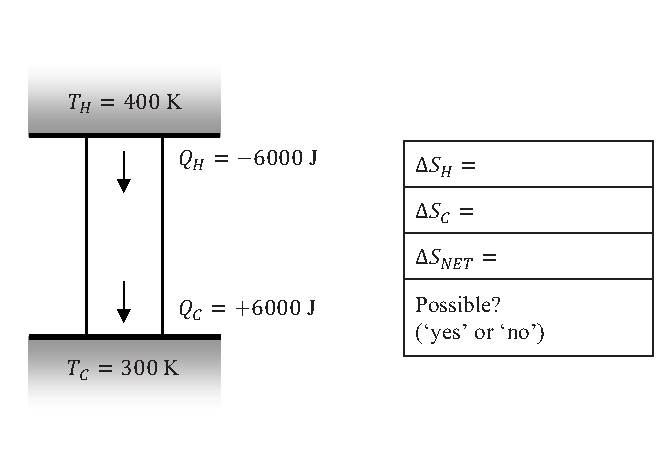
\includegraphics[width=0.5\textwidth]{entropy_is_it_possible/fig1.eps}
\vspace{-0.2 in}
\end{center}

(a) Use the expression for $\Delta S$ to fill in the table to the right of the figure with $\Delta S_H$ and $\Delta S_C$ for the hot and cold bricks.  Be careful with the signs for $Q_H$ and $Q_C$!  (We've dropped the ``$\Delta$'' from our notation for simplicity.)  Note that we're assuming here that both bricks are large enough that their temperatures remain roughly constant throughout the process; transferring 6000 Joules doesn't make a lot of difference to them.  Our lingo here is that those bodies are hot and cold ``reservoirs.''   
\answerspace{0.2 in}

(b) The net change in entropy $\Delta S_{NET}$ is the sum of $\Delta S_H$ and $\Delta S_C$.  Based on the sign of $\Delta S_{NET}$, is the process pictured above one that is actually possible in nature?
\answerspace{0.6 in}

\pagebreak[2]
Now consider the reverse process:

\begin{center}
\vspace{-0.2 in}
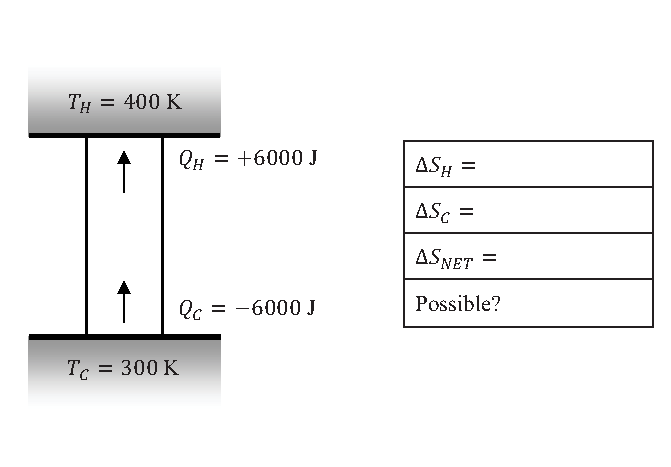
\includegraphics[width=0.5\textwidth]{entropy_is_it_possible/fig2.eps}
\vspace{-0.2 in}
\end{center}

(c) Fill in the table to the right of the figure above.   Could this process actually occur?  How do you know?
\answerspace{0.6 in}

\textbf{Activity 2: Extracting Work: Heat Engines}

There are many ways you can convert mechanical work $W$ into heat energy $Q$.  You can rub your hands together quickly to heat them with friction, or you can mechanically turn a generator to produce electricity and use it to power an electric heater.  Your experience tells you that using either of these methods to heat up a single brick doesn't break any physical laws.  In fact, the work $W$ you do has no direct bearing on $S_{NET}$, though the amount of heat $Q$ transferred does.

\begin{center}
\vspace{-0.2 in}
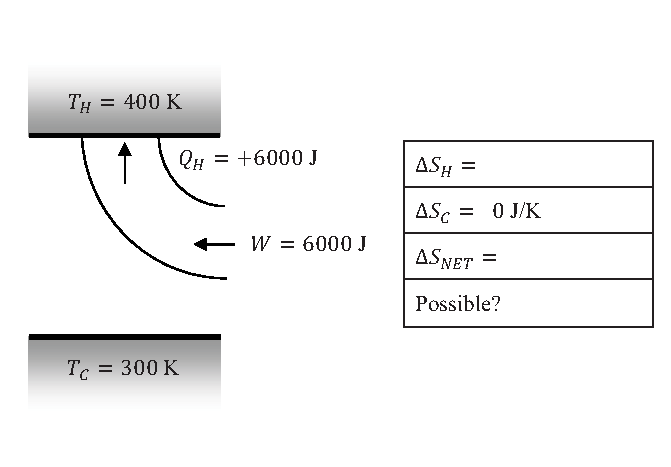
\includegraphics[width=0.5\textwidth]{entropy_is_it_possible/fig3.eps}
\vspace{-0.2 in}
\end{center}

(a) Fill in the table to the right of the figure.  Is the sign for $\Delta S$ consistent with whether this process can actually occur?
\answerspace{0.6 in}

\pagebreak[3]
Now consider the reverse process, in which heat energy is extracted from an object, and all of it is somehow transformed into useful mechanical work, like lifting some weights or generating electricity to do something else.

\begin{center}
\vspace{-0.2 in}
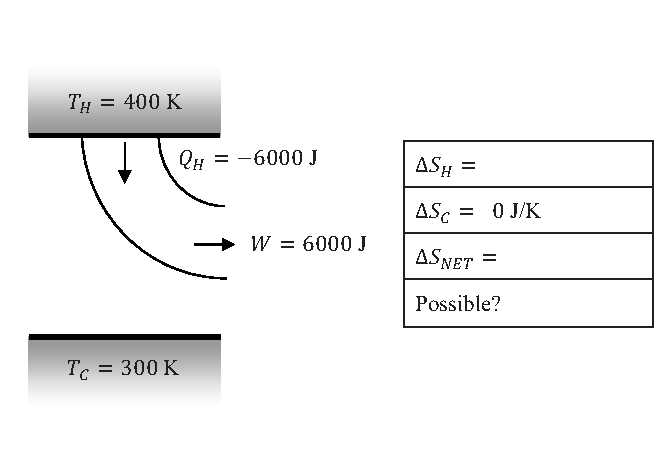
\includegraphics[width=0.5\textwidth]{entropy_is_it_possible/fig4.eps}
\vspace{-0.2 in}
\end{center}

(b) Fill in the table to the right of the figure.  Could this process actually occur? 
\answerspace{0.2 in}

But wait a second!  We \textit{know} that you can use heat from burning coal or from a nuclear reaction to turn water into steam, and that the steam can be used to turn a turbine on a generator.  This is where most of our electricity comes from!  \textit{Surely this is possible, right?}  The catch is that not all of the heat energy can be converted to work.  Some the heat from the steam must be transferred to a cold body, typically either to the atmosphere or to a large body of water.  

In the figure below, enough coal is burned to generate 6000 J of heat in a reservoir of steam.  Of the 6000 J transferred from the hot steam, 4800 J is dumped into the colder atmosphere, in the form of heat pouring from a smokestack, say.   

\begin{center}
\vspace{-0.3 in}
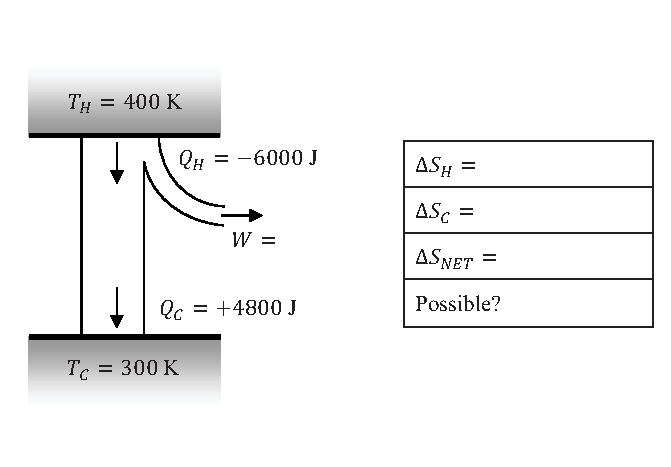
\includegraphics[width=0.5\textwidth]{entropy_is_it_possible/fig5.eps}
\vspace{-0.3 in}
\end{center}

(c) Fill in the table to the right of the figure, including the amount of work $W$ that is extracted.  Could the process actually occur, as shown?
\answerspace{0.2 in}

(d) The limiting case of a process that's theoretically \textit{just barely} possible is $\Delta S_{NET} = 0$.  Suppose that 6000 J is transferred from the hot reservoir.  What's the limit for the minimum $Q_C$ that must be transferred to the cold reservoir?
\answerspace{0.2 in}

(e) If  6000 J is transferred from the hot reservoir, what is the maximum work $W$ that can be extracted from the process?
\answerspace{0.2 in}

\pagebreak[2]
(f) Write a general expression for the maximum ratio of $W/Q_H$, in terms of only $T_H$ and $T_C$.  (Hint: start by writing $\Delta S = 0$ in terms of $Q_H$, $Q_C$, and the temperatures of the reservoirs.  Then use the idea of conservation of energy to write $Q_C$ in terms of $Q_H$ and $W$.)
\answerspace{1.5 in}

\textbf{Activity 3: Heating and Cooling Your House: Refrigerators and Heat Pumps}

Think of a hot summer day, when it's $100^\circ$F outside and your house is a stuffy $85^\circ$F inside.  

(a) If you open a window, is it possible that heat will spontaneously be transferred from inside your house to outside your house?  Why or why not?  (A diagram might help.  See Activity 1 if you're not sure.)
\answerspace{1.2 in}

(b) Is it possible to simply transform some thermal energy $Q$ from inside your house into mechanical work $W$?  Why or why not?  (Again, a diagram might help.  See Activity 2 if you're not sure.)
\answerspace{1.2 in}

The way to actually cool your house is to transfer some heat energy to the outside with the help of additional mechanical work, as shown below.  This is how an air conditioner works (more generally called a ``refrigerator'').

\begin{center}
\vspace{-0.3 in}
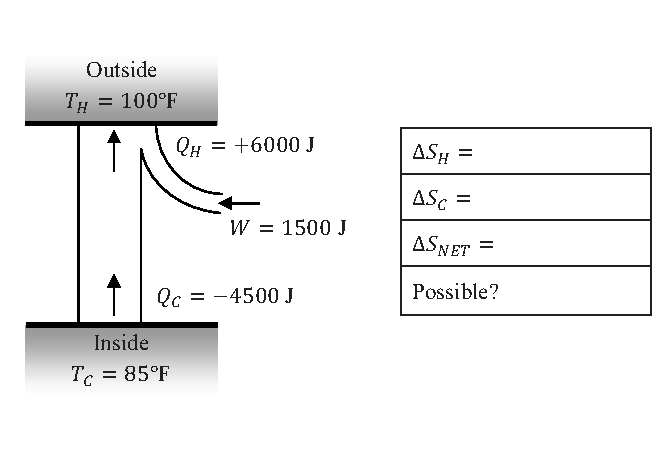
\includegraphics[width=0.5\textwidth]{entropy_is_it_possible/fig6.eps}
\vspace{-0.4 in}
\end{center}

(c) Fill in the table to the right of the figure, including the heat energy $Q_H$, to show that the situation above is possible for the quantities given.  (Yes, you have to convert from Fahrenheit to Kelven.)
\answerspace{0.2 in}

\pagebreak[2]
Finally, suppose you want to heat your house in the winter when it's $65^\circ$F inside and $50^\circ$F outside.  The diagrams below show two possible ways to do it.  On the left is a simple space heater, in which work is converted to heat energy.  On the right is a ``heat pump,'' which is basically the same as the air conditioner, but with the inside and outside flipped.  In each case, you are putting 6000 J of heat energy into the house.

\begin{center}
\vspace{-0.2 in}
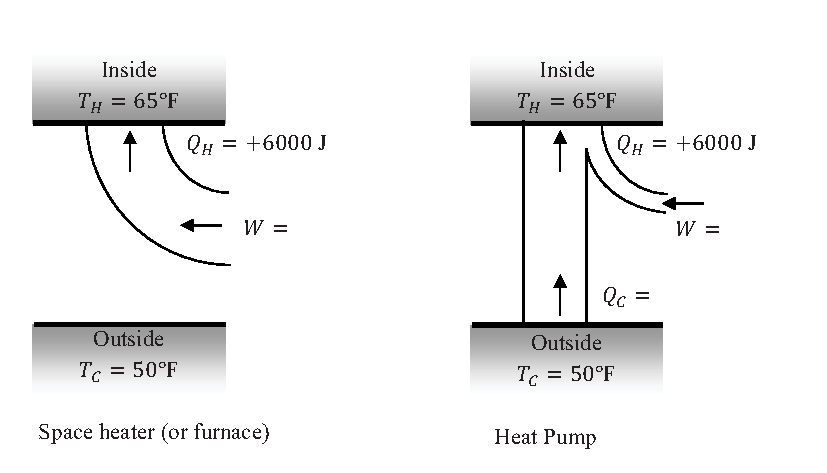
\includegraphics[width=0.5\textwidth]{entropy_is_it_possible/fig7.eps}
\vspace{-0.1 in}
\end{center}

(d) The theoretical maximum efficiency of the heat pump would be when $\Delta S_{NET}=0$.  What would $Q_C$ need to be then?
\answerspace{1.2 in}

(e) If the heat pump is at that maximum theoretical efficiency, how much work $W$ is required for $Q_H = 6000$ J?
 \answerspace{0.6 in}

(f) By contrast, how much work $W$ does the simple space heater need to do the same job? 
\answerspace{0.4 in}

(g) How cool is that?
\answerspace{0.4 in}

(h) If the outside temperature were colder, would the advantage of the heat pump over the simple space heater increase or decrease? 
\answerspace{0.4 in}

In real life, heat pumps aren't quite as efficient as the maximum theoretical efficiency you assumed here.  And as you noted above, they get worse when the outside temperature gets colder.  (They also usually run on electricity, and the cost per Joule for electrical power is generally higher than for natural gas.)  Nevertheless, houses in moderate climates like Virginia and further south often have heat pumps, sometimes in addition to traditional gas furnaces.  The heat pump warms the house economically in the fall and spring, and a thermostat trips the gas furnace to kick on when the outside temperature falls below about $40^\circ$F.


%--------------------------------------------
\appendix
\setcounter{section}{4} %set this counter to number MINUS ONE corresponding to desired appendix letter. (4 for `E', etc.)
%Put include statements for supplementary appendices below here.
\end{document}
